\subsection{Опис власних тестiв}

Для реалізації алгоритму LUOV проводились наступні тести:

\begin{itemize}[label={$\bullet$}]
    \item Тест на швидкодію в залежності від розміру вхідного повідомлення. \\
    Для тесту використовувались повідомлення різних розмірів (100 символів, 1000 символів та 10000 символів). В результаті було отримано, що швидкодія підписання та перевірки підпису не залежить від довжини вхідного повідомлення. Середня швидкодія при виконанні даного тесту лежить в межах проміжку [600,900] мс.
    \item Тест генерації підпису. \\
    В результаті було отримано правильний підпис для повідомлення.
    \item Тест верифікації підпису повідомлення. \\
    В результаті було отримано значення true після верифікації підпису для повідомлення.
    \item Тест верифікації пошкодженого повідомлення. \\
    В результаті було отримано значення false після верифікації підпису для пошкодженого повідомлення.
    \item Тест використання різних параметрів кривої.
    В результаті було показано використання алгоритму підпису LUOV для 2-ох можливих варіантів набору параметрів.
\end{itemize}

\subsection{Детальний опис особливостей реалiзацiї та приклади застосування}

При реалізації алгориму цифрового підпису LUOV посилалися на деякі інші відомі реалізації алгоритму, включно з документацією. Ось деякі з них:
\begin{enumerate}
    \item \url{https://github.com/WardBeullens/LUOV}
    \item \url{https://github.com/saadislamm/QuantumHammer}
    \item \url{https://github.com/Danny-xyy/LUOV}
    \item \url{https://github.com/EddAngulo/luov_java_implementation}
    \item \url{https://github.com/WardBeullens/ThesisCode}
\end{enumerate}

\vspace{0.5cm}
\textbf{Основні функції реалізації алгоритму}:
\begin{enumerate}
    \item Можливість вибору поля з параметрами для роботи з алгоритмом серед запропонованих:
    \begin{itemize}
        \item GF(207): r=7,m=57,v=197.
        \item GF(261): r=61,m=60,v=261.
    \end{itemize}
    \item Функція генерації публічного та приватного ключів: keyGen().
    \item Функція генерації підпису повідомлення: sign().
    \item Функція перевірки підписаного повідомлення: verify(). 
\end{enumerate}

\vspace{0.5cm}
\textbf{\LargeПриклади використання реалізації та проведених тестів:}

% \vspace{-0.5cm}
\begin{figure}[ht]
    \centering
    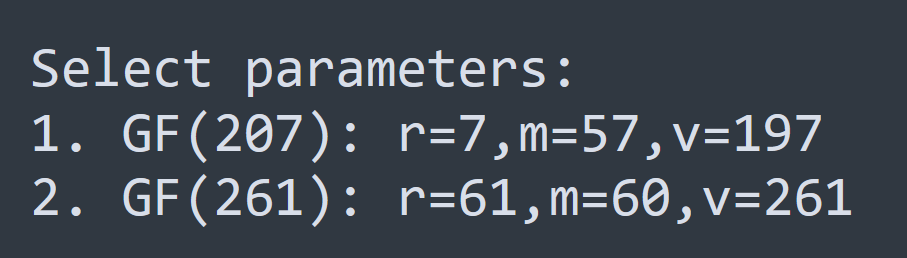
\includegraphics[scale = 0.55]{IMAGES/select_parameters.png}
    \caption{Можливість вибору параметрів.}
    \label{fig1}
\end{figure}

\begin{figure}[ht]
    \centering
    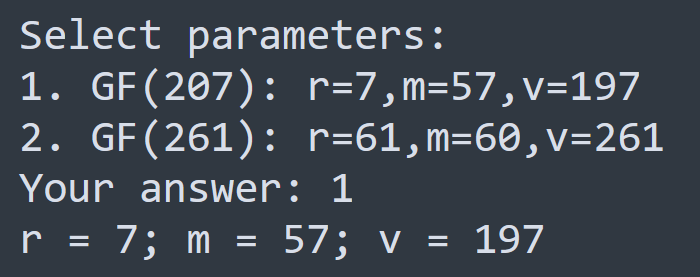
\includegraphics[scale = 0.7]{IMAGES/select_param1.png}
    \caption{Вибір 1-го типу параметрів.}
    \label{fig1}
\end{figure}

\begin{figure}[ht]
    \centering
    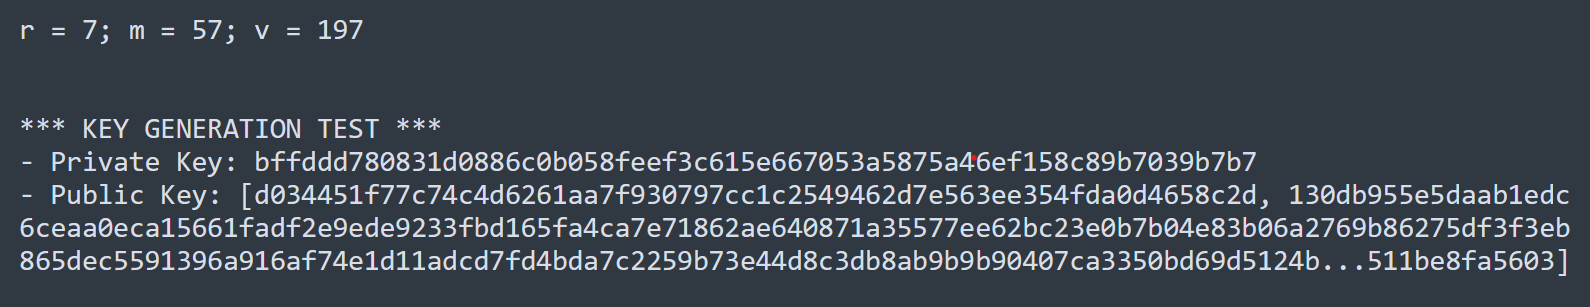
\includegraphics[scale = 0.6]{IMAGES/key_gen1.png}
    \caption{Генерація ключів для 1-го типу параметрів.}
    \label{fig1}
\end{figure}

\begin{figure}[ht]
    \centering
    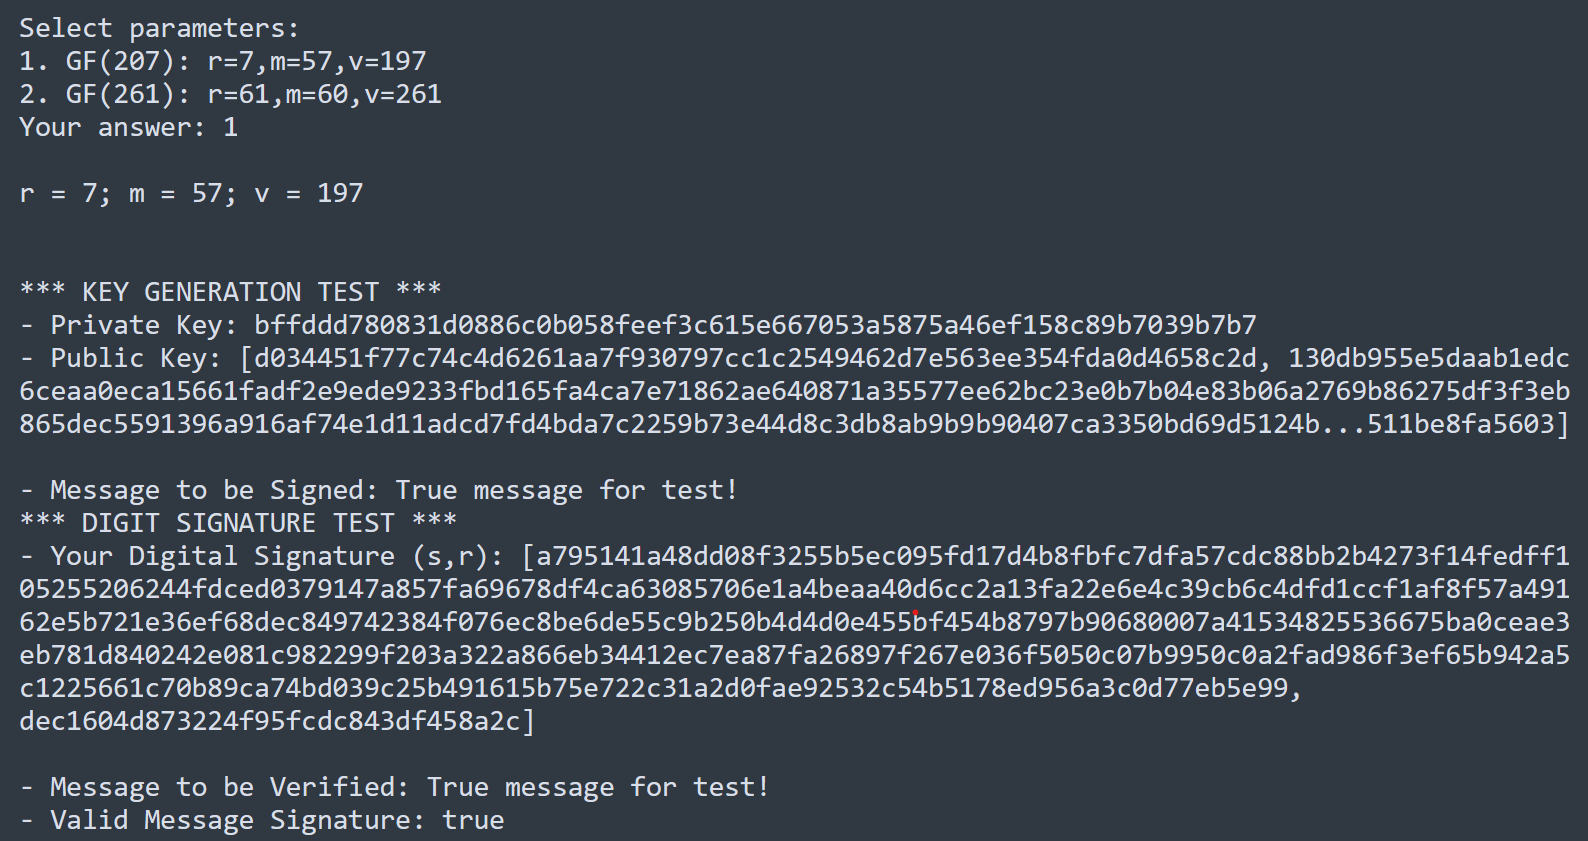
\includegraphics[scale = 0.53]{IMAGES/digit_sign_testT1.png}
    \caption{\largeПідписування повідомлення для 1-го типу параметрів.}
    \label{fig1}
\end{figure}
% \vspace{2cm}
\begin{figure}[ht]
    \centering
    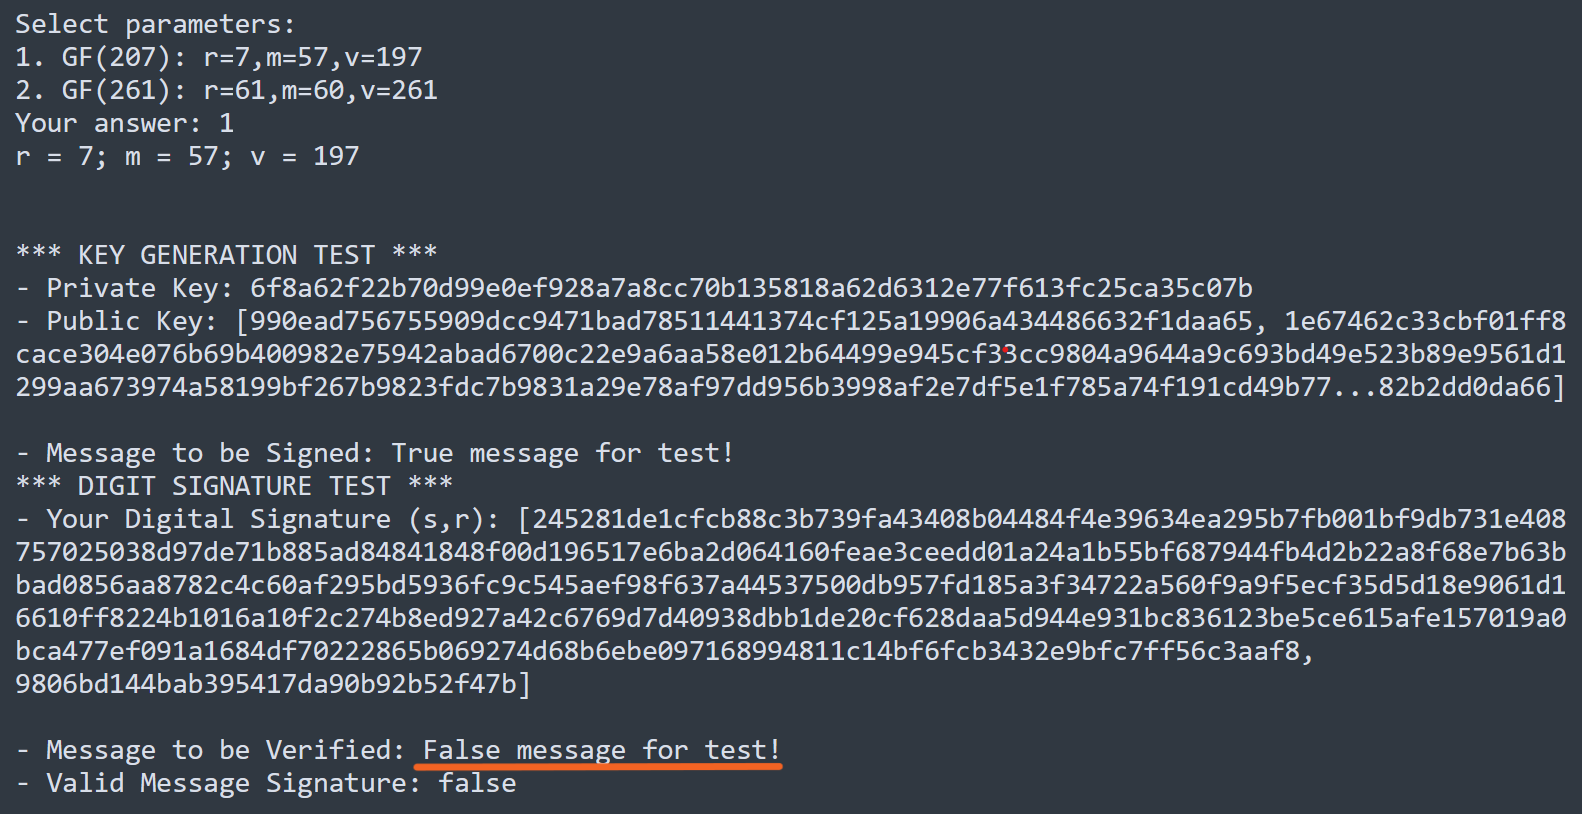
\includegraphics[scale = 0.53]{IMAGES/digit_sign_testF1.png}
    \caption{\largeПошкодження повідомлення при верифікації для 1-го типу параметрів.}
    \label{fig1}
\end{figure}

\begin{figure}[ht]
    \centering
    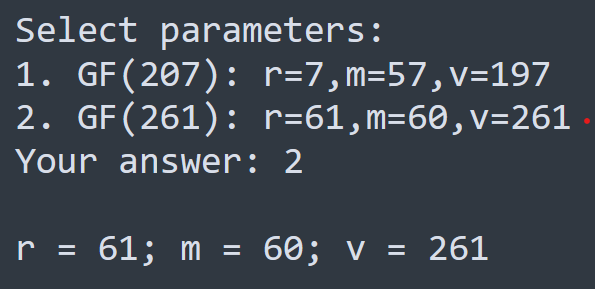
\includegraphics[scale = 0.7]{IMAGES/select_param2.png}
    \caption{Вибір 2-го типу параметрів.}
    \label{fig1}
\end{figure}

\begin{figure}[ht]
    \centering
    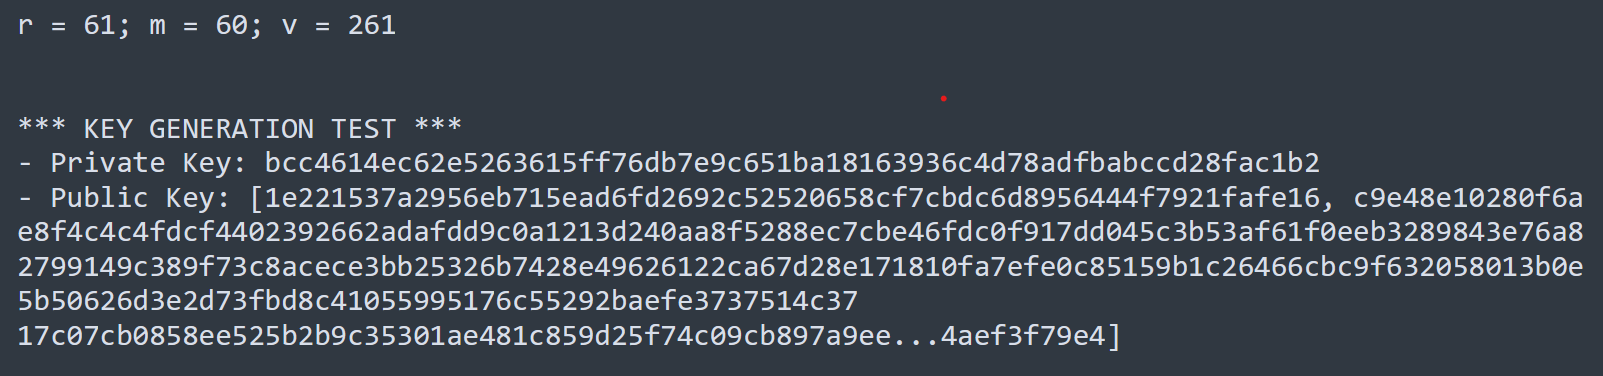
\includegraphics[scale = 0.6]{IMAGES/key_gen2.png}
    \caption{Генерація ключів для 2-го типу параметрів.}
    \label{fig1}
\end{figure}

\begin{figure}[ht!]
    \centering
    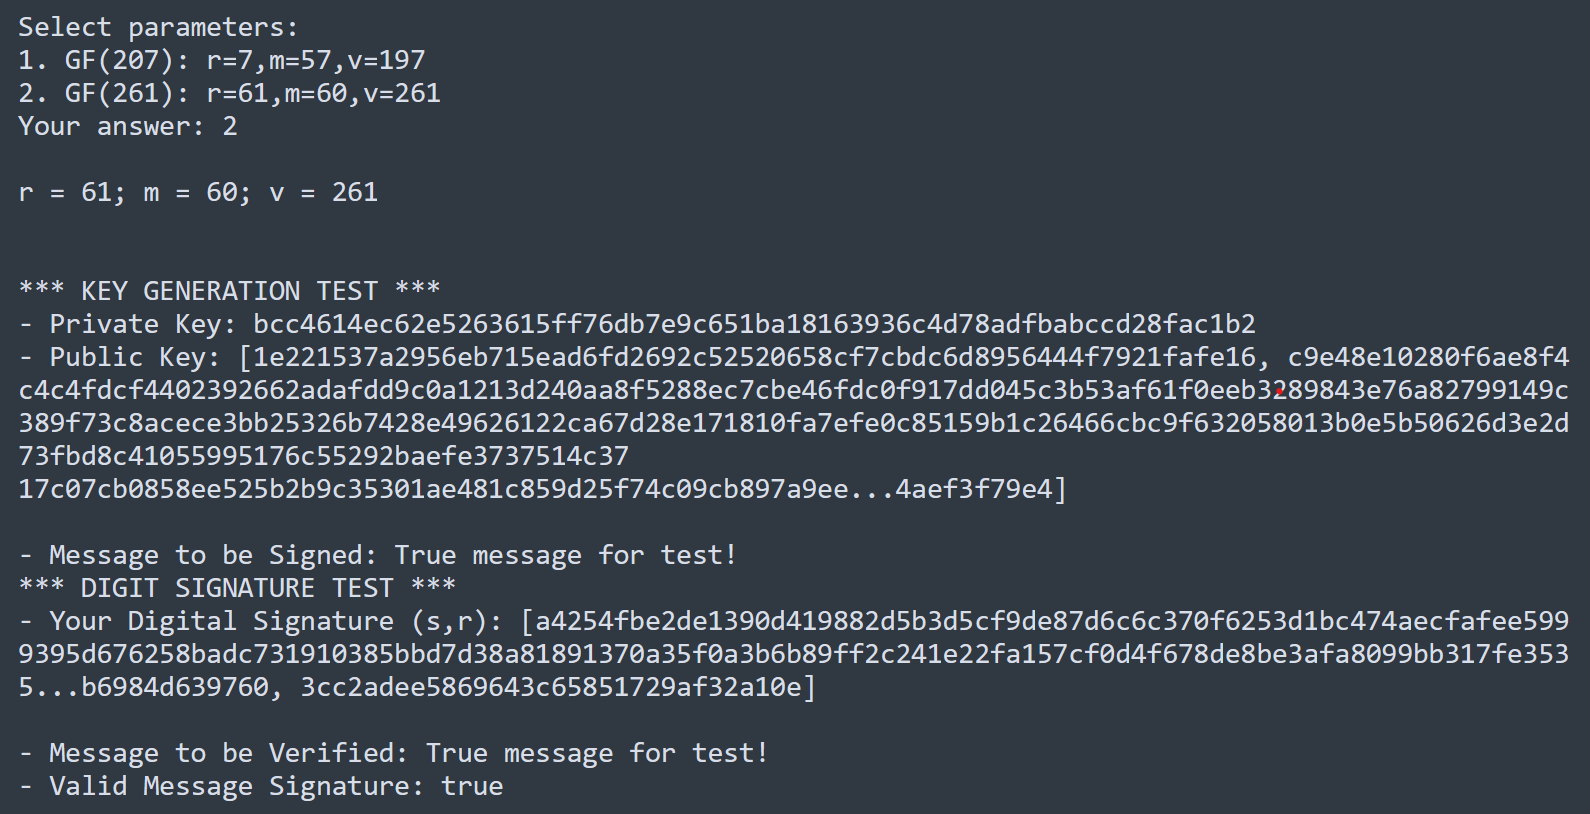
\includegraphics[scale = 0.6]{IMAGES/digit_sign_testT2.png}
    \caption{\largeПідписування повідомлення для 2-го типу параметрів.}
    \label{fig1}
\end{figure}

\newpage
А також прикріплюємо результат тесту верифікації підпису з пошкодженим повідомленням для 2-го типу параметрів кривої:

\begin{figure}[ht!]
    \centering
    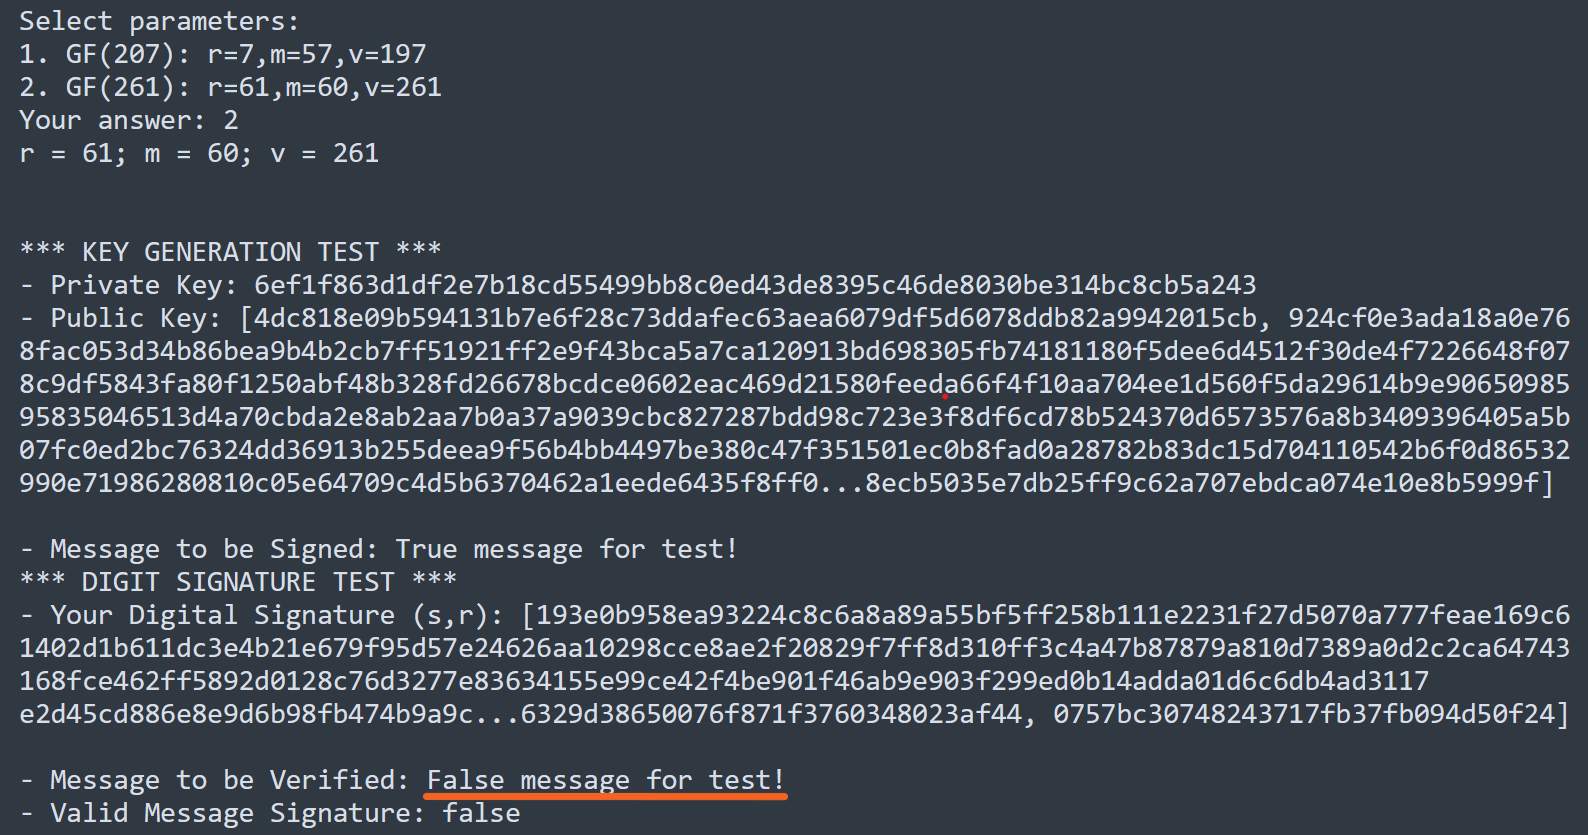
\includegraphics[scale = 0.6]{IMAGES/digit_sign_testF2.png}
    \caption{\largeПошкодження повідомлення при верифікації для 2-го типу параметрів.}
    \label{fig1}
\end{figure}

\newpage
\subsection{Результати аналiзу постквантової стiйкостi}
\vspace{-0.5cm}
Постквантову стійкість можна перевірити оцінкою складності прямої атаки на LUOV з одним з можливих наборів параметрів, наприклад (r = 7, m = 57, v = 197); можемо визначити рівень безпеки, який досягає цей набір. Для цього можна скористатися використанням методу Тома і Вольфа. Таким чином можна звести пошук розв'язку цієї недовизначеної системи до пошуку розв'язку детермінованої системи з $57+1-\lfloor(57+197)/57\rfloor$ = 54 рівняння. Ми припускаємо, що ця система та системи, отримані шляхом фіксації ряду змінних, є напіврегулярними. Якщо ми фіксуємо k додаткових змінних, то ступінь регулярності дорівнює ступеню першого члена в степеневому ряді:

$S_{54,54-k}(x) = \frac{(1-x^2)^{54}}{(1-x)^{54-k}}$, який має недодатний коефіцієнт.\\
Для k = 0 ми маємо $S_{54}(x)$ = $(1 + x)54$, тому ступінь регулярності дорівнює 55.
Продовжуючи обчислення далі визначимо, що складність прямої атаки перевищує нижню межу 2146×1,1, як вимагається.
А якщо використати пошук Гровера замість частини гібридного підходу грубої сили, щоб прискорити пряму атаку. Таким чином продовжуючи обчислення далі дійдемо до того, що для всіх вибраних параметрів і всіх практичних значень k складність навіть одного обчислення базису Гробнера перевищує 264, і алгоритм Гровера повинен виконувати велику кількість цих обчислень послідовно, щоб отримати помітне прискорення порівняно з класичним грубим методом. 

В результаті отримаємо, що алгоритм LUOV має постквантову стійкість до атак.